%% ma: L12-B08-0022
%% lop: 12
%% chuong: 2
%% bai: 8
%% dang: 12.8.14
%% loai: TLN
%% muc: VD
%% dap_an: "17,2"
%% nguon: "(NBV)-ĐỀ SỐ 15-MỖI NGÀY 1 ĐỀ THI 2025.pdf (D15, MỖI NGÀY 1 ĐỀ - Đề số 15), Phần III Câu 6"
%% kien_thuc: "Bài 7-8 (tọa độ hóa, điều kiện bốn điểm đồng phẳng với vectơ trong không gian)"
%% trang_thai: chinh-thuc
%% ghi_chu: "Đã duyệt 16/10/2026. Đáp án gốc 17,2 đúng (kiểm bằng sympy). Hình dựng lại từ số liệu của đề: hình thang vuông ABCD, AB = 25, AD = 15, BC = 18 (vẽ gần đúng tỉ lệ). Bỏ họa tiết nền sân (ảnh trang trí)."
\begin{ex}
Một phần sân trường được định vị bởi các điểm $A,B,C,D$ như hình vẽ. Bước đầu chúng được lấy ``thăng bằng'' để có cùng độ cao so với mặt đất, biết $ABCD$ là hình thang vuông ở $A$ và $B$ với độ dài $AB=25\ \mathrm m$, $AD=15\ \mathrm m$, $BC=18\ \mathrm m$. Do yêu cầu kĩ thuật, khi lát phẳng phần sân trường phải thoát nước về góc sân ở $C$ nên người ta lấy độ cao ở các điểm $B,C,D$ lần lượt xuống thấp hơn so với độ cao ở $A$ là $10\ \mathrm{cm}$, $a\ \mathrm{cm}$, $6\ \mathrm{cm}$ tương ứng sao cho bốn điểm $A,B',C',D'$ đồng phẳng. Tìm giá trị của $a$.
\begin{center}
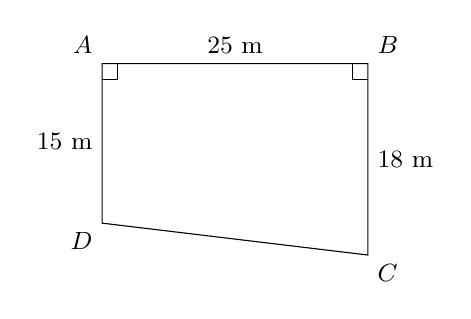
\begin{tikzpicture}[scale=.9]
  \draw (0,0)--(3.75,0)--(3.75,-2.7)--(0,-2.25)--cycle;
  \node[above left,font=\small] at (0,0) {$A$};
  \node[above right,font=\small] at (3.75,0) {$B$};
  \node[below right,font=\small] at (3.75,-2.7) {$C$};
  \node[below left,font=\small] at (0,-2.25) {$D$};
  \node[above,font=\small] at (1.875,0) {$25\ \mathrm m$};
  \node[left,font=\small] at (0,-1.1) {$15\ \mathrm m$};
  \node[right,font=\small] at (3.75,-1.35) {$18\ \mathrm m$};
  \draw (0,-.22)--(.22,-.22)--(.22,0) (3.53,0)--(3.53,-.22)--(3.75,-.22);\end{tikzpicture}
\end{center}
\shortans{17,2}
\loigiai{Chọn hệ trục $Axyz$ với $A(0;0;0)$, $B(25;0;0)$, $D(0;15;0)$, $C(25;18;0)$, trục $Az$ hướng lên; đổi độ cao ra mét: $B'(25;0;-0{,}1)$, $D'(0;15;-0{,}06)$, $C'(25;18;-0{,}01a)$.

Mặt phẳng $(AB'D')$ có dạng $z=px+qy$ với $25p=-0{,}1$, $15q=-0{,}06$, suy ra $p=q=-0{,}004$.

$C'$ thuộc mặt phẳng nên $-0{,}01a=25p+18q=-0{,}1-0{,}072=-0{,}172$, suy ra $a=17{,}2$.}
\end{ex}
